% Options for packages loaded elsewhere
\PassOptionsToPackage{unicode}{hyperref}
\PassOptionsToPackage{hyphens}{url}
%
\documentclass[
  english,
]{book}
\usepackage{amsmath,amssymb}
\usepackage{lmodern}
\usepackage{ifxetex,ifluatex}
\ifnum 0\ifxetex 1\fi\ifluatex 1\fi=0 % if pdftex
  \usepackage[T1]{fontenc}
  \usepackage[utf8]{inputenc}
  \usepackage{textcomp} % provide euro and other symbols
\else % if luatex or xetex
  \usepackage{unicode-math}
  \defaultfontfeatures{Scale=MatchLowercase}
  \defaultfontfeatures[\rmfamily]{Ligatures=TeX,Scale=1}
\fi
% Use upquote if available, for straight quotes in verbatim environments
\IfFileExists{upquote.sty}{\usepackage{upquote}}{}
\IfFileExists{microtype.sty}{% use microtype if available
  \usepackage[]{microtype}
  \UseMicrotypeSet[protrusion]{basicmath} % disable protrusion for tt fonts
}{}
\makeatletter
\@ifundefined{KOMAClassName}{% if non-KOMA class
  \IfFileExists{parskip.sty}{%
    \usepackage{parskip}
  }{% else
    \setlength{\parindent}{0pt}
    \setlength{\parskip}{6pt plus 2pt minus 1pt}}
}{% if KOMA class
  \KOMAoptions{parskip=half}}
\makeatother
\usepackage{xcolor}
\IfFileExists{xurl.sty}{\usepackage{xurl}}{} % add URL line breaks if available
\IfFileExists{bookmark.sty}{\usepackage{bookmark}}{\usepackage{hyperref}}
\hypersetup{
  pdftitle={ReCentering Psych Stats: Multilevel/Hierarchical Linear Modeling},
  pdfauthor={Lynette H Bikos, PhD, ABPP},
  pdflang={en},
  hidelinks,
  pdfcreator={LaTeX via pandoc}}
\urlstyle{same} % disable monospaced font for URLs
\usepackage{color}
\usepackage{fancyvrb}
\newcommand{\VerbBar}{|}
\newcommand{\VERB}{\Verb[commandchars=\\\{\}]}
\DefineVerbatimEnvironment{Highlighting}{Verbatim}{commandchars=\\\{\}}
% Add ',fontsize=\small' for more characters per line
\usepackage{framed}
\definecolor{shadecolor}{RGB}{248,248,248}
\newenvironment{Shaded}{\begin{snugshade}}{\end{snugshade}}
\newcommand{\AlertTok}[1]{\textcolor[rgb]{0.94,0.16,0.16}{#1}}
\newcommand{\AnnotationTok}[1]{\textcolor[rgb]{0.56,0.35,0.01}{\textbf{\textit{#1}}}}
\newcommand{\AttributeTok}[1]{\textcolor[rgb]{0.77,0.63,0.00}{#1}}
\newcommand{\BaseNTok}[1]{\textcolor[rgb]{0.00,0.00,0.81}{#1}}
\newcommand{\BuiltInTok}[1]{#1}
\newcommand{\CharTok}[1]{\textcolor[rgb]{0.31,0.60,0.02}{#1}}
\newcommand{\CommentTok}[1]{\textcolor[rgb]{0.56,0.35,0.01}{\textit{#1}}}
\newcommand{\CommentVarTok}[1]{\textcolor[rgb]{0.56,0.35,0.01}{\textbf{\textit{#1}}}}
\newcommand{\ConstantTok}[1]{\textcolor[rgb]{0.00,0.00,0.00}{#1}}
\newcommand{\ControlFlowTok}[1]{\textcolor[rgb]{0.13,0.29,0.53}{\textbf{#1}}}
\newcommand{\DataTypeTok}[1]{\textcolor[rgb]{0.13,0.29,0.53}{#1}}
\newcommand{\DecValTok}[1]{\textcolor[rgb]{0.00,0.00,0.81}{#1}}
\newcommand{\DocumentationTok}[1]{\textcolor[rgb]{0.56,0.35,0.01}{\textbf{\textit{#1}}}}
\newcommand{\ErrorTok}[1]{\textcolor[rgb]{0.64,0.00,0.00}{\textbf{#1}}}
\newcommand{\ExtensionTok}[1]{#1}
\newcommand{\FloatTok}[1]{\textcolor[rgb]{0.00,0.00,0.81}{#1}}
\newcommand{\FunctionTok}[1]{\textcolor[rgb]{0.00,0.00,0.00}{#1}}
\newcommand{\ImportTok}[1]{#1}
\newcommand{\InformationTok}[1]{\textcolor[rgb]{0.56,0.35,0.01}{\textbf{\textit{#1}}}}
\newcommand{\KeywordTok}[1]{\textcolor[rgb]{0.13,0.29,0.53}{\textbf{#1}}}
\newcommand{\NormalTok}[1]{#1}
\newcommand{\OperatorTok}[1]{\textcolor[rgb]{0.81,0.36,0.00}{\textbf{#1}}}
\newcommand{\OtherTok}[1]{\textcolor[rgb]{0.56,0.35,0.01}{#1}}
\newcommand{\PreprocessorTok}[1]{\textcolor[rgb]{0.56,0.35,0.01}{\textit{#1}}}
\newcommand{\RegionMarkerTok}[1]{#1}
\newcommand{\SpecialCharTok}[1]{\textcolor[rgb]{0.00,0.00,0.00}{#1}}
\newcommand{\SpecialStringTok}[1]{\textcolor[rgb]{0.31,0.60,0.02}{#1}}
\newcommand{\StringTok}[1]{\textcolor[rgb]{0.31,0.60,0.02}{#1}}
\newcommand{\VariableTok}[1]{\textcolor[rgb]{0.00,0.00,0.00}{#1}}
\newcommand{\VerbatimStringTok}[1]{\textcolor[rgb]{0.31,0.60,0.02}{#1}}
\newcommand{\WarningTok}[1]{\textcolor[rgb]{0.56,0.35,0.01}{\textbf{\textit{#1}}}}
\usepackage{longtable,booktabs,array}
\usepackage{calc} % for calculating minipage widths
% Correct order of tables after \paragraph or \subparagraph
\usepackage{etoolbox}
\makeatletter
\patchcmd\longtable{\par}{\if@noskipsec\mbox{}\fi\par}{}{}
\makeatother
% Allow footnotes in longtable head/foot
\IfFileExists{footnotehyper.sty}{\usepackage{footnotehyper}}{\usepackage{footnote}}
\makesavenoteenv{longtable}
\usepackage{graphicx}
\makeatletter
\def\maxwidth{\ifdim\Gin@nat@width>\linewidth\linewidth\else\Gin@nat@width\fi}
\def\maxheight{\ifdim\Gin@nat@height>\textheight\textheight\else\Gin@nat@height\fi}
\makeatother
% Scale images if necessary, so that they will not overflow the page
% margins by default, and it is still possible to overwrite the defaults
% using explicit options in \includegraphics[width, height, ...]{}
\setkeys{Gin}{width=\maxwidth,height=\maxheight,keepaspectratio}
% Set default figure placement to htbp
\makeatletter
\def\fps@figure{htbp}
\makeatother
\setlength{\emergencystretch}{3em} % prevent overfull lines
\providecommand{\tightlist}{%
  \setlength{\itemsep}{0pt}\setlength{\parskip}{0pt}}
\setcounter{secnumdepth}{5}
\usepackage{booktabs}
\ifxetex
  % Load polyglossia as late as possible: uses bidi with RTL langages (e.g. Hebrew, Arabic)
  \usepackage{polyglossia}
  \setmainlanguage[]{english}
\else
  \usepackage[main=english]{babel}
% get rid of language-specific shorthands (see #6817):
\let\LanguageShortHands\languageshorthands
\def\languageshorthands#1{}
\fi
\ifluatex
  \usepackage{selnolig}  % disable illegal ligatures
\fi
\usepackage[]{natbib}
\bibliographystyle{plainnat}

\title{ReCentering Psych Stats: Multilevel/Hierarchical Linear Modeling}
\author{Lynette H Bikos, PhD, ABPP}
\date{}

\begin{document}
\maketitle

{
\setcounter{tocdepth}{1}
\tableofcontents
}
\hypertarget{book-cover}{%
\chapter*{BOOK COVER}\label{book-cover}}
\addcontentsline{toc}{chapter}{BOOK COVER}

\begin{figure}
\centering
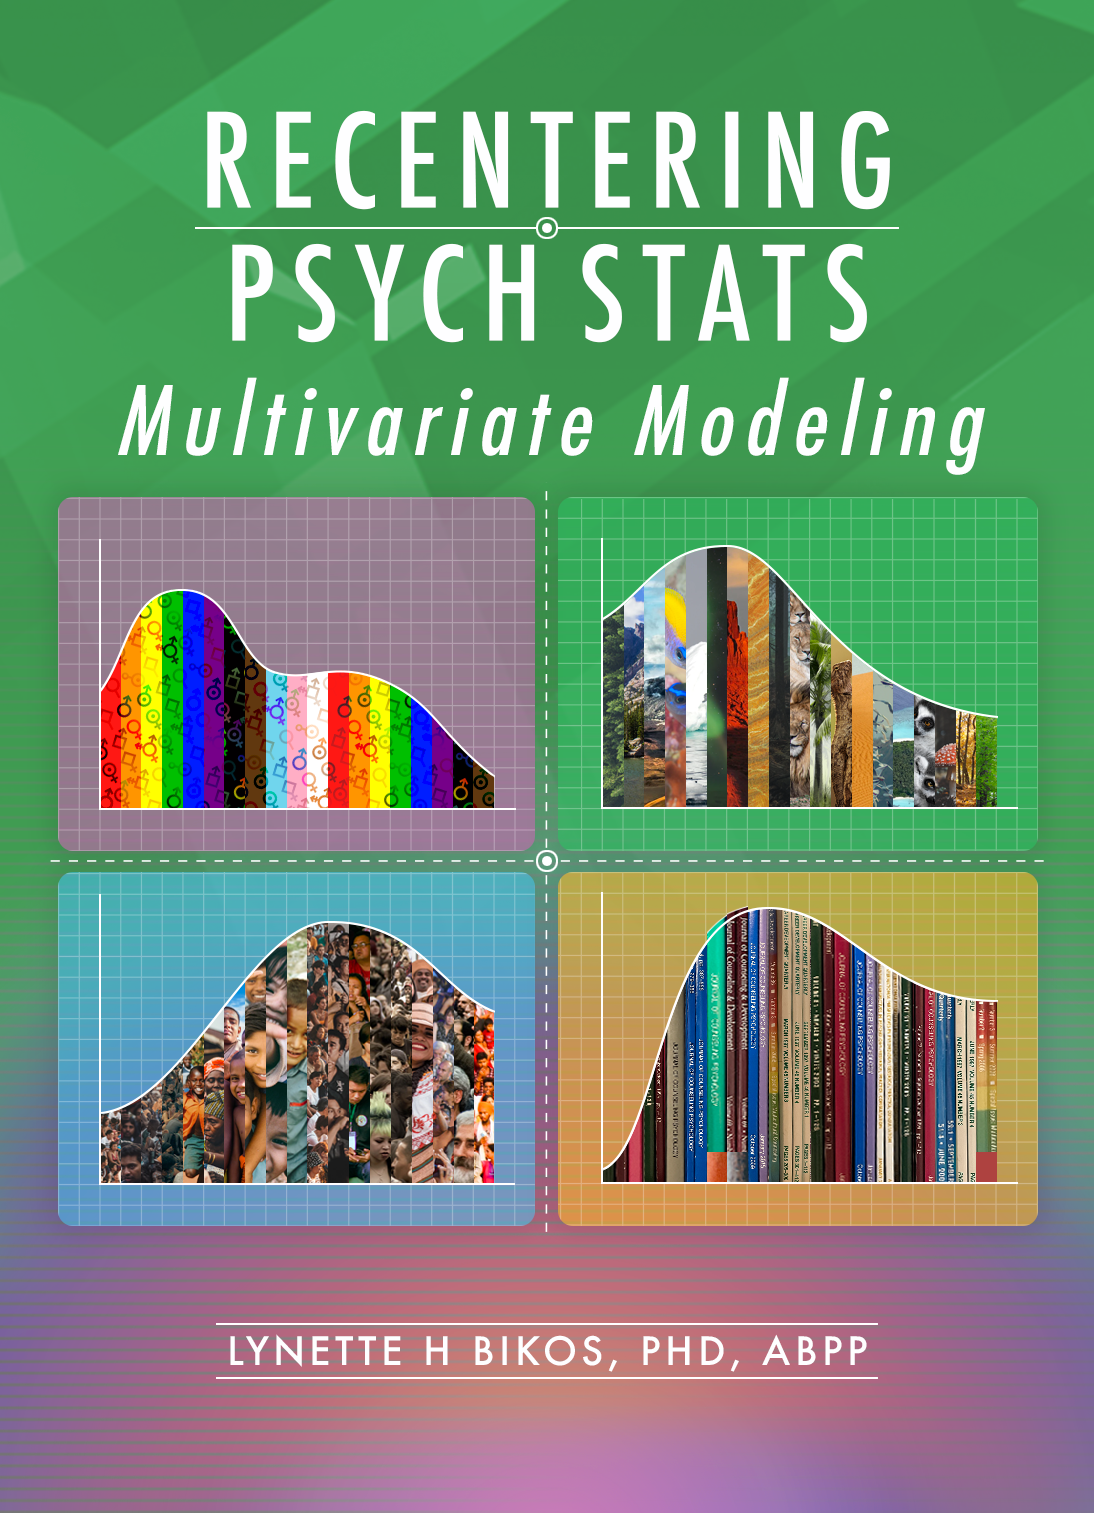
\includegraphics{images/ReC_multivariate_bkcvr.png}
\caption{An image of the book cover. It includes four quadrants of non-normal distributions representing gender, race/ethnicty, sustainability/global concerns, and journal articles}
\end{figure}

\hypertarget{preface}{%
\chapter*{PREFACE}\label{preface}}
\addcontentsline{toc}{chapter}{PREFACE}

\textbf{If you are viewing this document, you should know that this is a book-in-progress. Early drafts are released for the purpose teaching my classes and gaining formative feedback from a host of stakeholders. The document was last updated on 06 May 2021}

\href{https://spu.hosted.panopto.com/Panopto/Pages/Viewer.aspx?id=c932455e-ef06-444a-bdca-acf7012d759a}{Screencasted Lecture Link}

To \emph{center} a variable in regression means to set its value at zero and interpret all other values in relation to this reference point. Regarding race and gender, researchers often center male and White at zero. Further, it is typical that research vignettes in statistics textbooks are similarly seated in a White, Western (frequently U.S.), heteronormative, framework. The purpose of this project is to create a set of open educational resources (OER) appropriate for doctoral and post-doctoral training that contribute to a socially responsive pedagogy -- that is, it contributes to justice, equity, diversity, and inclusion.

Statistics training in doctoral programs are frequently taught with fee-for-use programs (e.g., SPSS/AMOS, SAS, MPlus) that may not be readily available to the post-doctoral professional. In recent years, there has been an increase and improvement in R packages (e.g., \emph{psych}, \emph{lavaan}) used for in analyses common to psychological research. Correspondingly, many graduate programs are transitioning to statistics training in R (free and open source). This is a challenge for post-doctoral psychologists who were trained with other software. This OER will offer statistics training with R and be freely available (specifically in a GitHub respository and posted through GitHub Pages) under a Creative Commons Attribution - Non Commercial - Share Alike license {[}CC BY-NC-SA 4.0{]}.

Training models for doctoral programs in HSP are commonly scholar-practitioner, scientist-practitioner, or clinical-scientist. An emerging model, the \emph{scientist-practitioner-advocacy} training model incorporates social justice advocacy so that graduates are equipped to recognize and address the sociocultural context of oppression and unjust distribution of resources and opportunities \citep{mallinckrodt_scientist-practitioner-advocate_2014}. In statistics textbooks, the use of research vignettes engages the learner around a tangible scenario for identifying independent variables, dependent variables, covariates, and potential mechanisms of change. Many students recall examples in Field's \citeyearpar{field_discovering_2012} popular statistics text: Viagra to teach one-way ANOVA, beer goggles for two-way ANOVA, and bushtucker for repeated measures. What if the research vignettes were more socially responsive?

In this OER, research vignettes will be from recently published articles where:

\begin{itemize}
\tightlist
\item
  the author's identity is from a group where scholarship is historically marginalized (e.g., BIPOC, LGBTQ+, LMIC{[}low-middle income countries{]}),
\item
  the research is responsive to issues of justice, equity, inclusion, diversity,
\item
  the lesson's statistic is used in the article, and
\item
  there is sufficient information in the article to simulate the data for the chapter example(s) and practice problem(s); or it is publicly available.
\end{itemize}

In training for multicultural competence, the saying, ``A fish doesn't know that it's wet'' is often used to convey the notion that we are often unaware of our own cultural characteristics. In recent months and years, there has been an increased awakening to the institutional and systemic racism that our systems are perpetuating. Queuing from the water metaphor, I am hopeful that a text that is recentered in the ways I have described can contribute to \emph{changing the water} in higher education and in the profession of psychology.

\hypertarget{copyright-with-open-access}{%
\section*{Copyright with Open Access}\label{copyright-with-open-access}}
\addcontentsline{toc}{section}{Copyright with Open Access}

This book is published under a a Creative Commons Attribution-NonCommercial-ShareAlike 4.0 International License. This means that this book can be reused, remixed, retained, revised and redistributed (including commercially) as long as appropriate credit is given to the authors. If you remix, or modify the original version of this open textbook, you must redistribute all versions of this open textbook under the same license - CC BY-SA.

A \href{https://github.com/lhbikos/ReC_MultivariateModeling}{GitHub open-source repository} contains all of the text and source code for the book, including data and images.

\hypertarget{acknowledgements}{%
\chapter*{ACKNOWLEDGEMENTS}\label{acknowledgements}}
\addcontentsline{toc}{chapter}{ACKNOWLEDGEMENTS}

As a doctoral student at the University of Kansas (1992-2005), I learned that ``a foreign language'' was required for graduation. \emph{Please note that as one who studies the intersections of global, vocational, and sustainable psychology, I regret that I do not have language skills beyond English.} This could have been met with credit from high school my rural, mid-Missouri high school did not offer such classes. This requirement would have typically been met with courses taken during an undergraduate program -- but my non-teaching degree in the University of Missouri's School of Education was exempt from this. The requirement could have also been met with a computer language (fortran, C++) -- I did not have any of those either. There was a tiny footnote on my doctoral degree plan that indicated that a 2-credit course, ``SPSS for Windows'' would substitute for the language requirement. Given that it was taught by my one of my favorite professors, I readily signed up. As it turns out, Samuel B. Green, PhD, was using the course to draft chapters in the textbook \citep{green_using_2014} that has been so helpful for so many. Unfortunately, Drs. Green (1947 - 2018) and Salkind (2947 - 2017) are no longer with us. I have worn out numerous versions of their text. Another favorite text of mine was Dr.~Barbara Byrne's \citeyearpar{byrne_structural_2016}, ``Structural Equation Modeling with AMOS.'' I loved the way she worked through each problem and paired it with a published journal article, so that the user could see how the statistical evaluation fit within the larger project/article. I took my tea-stained text with me to a workshop she taught at APA and was proud of the signature she added to it (a little catfur might have fallen out). Dr.~Byrne created SEM texts for a number of statistical programs (e.g., LISREL, EQS, MPlus). As I was learning R, I wrote Dr.~Byrne, asking if she had an edition teaching SEM/CFA with R. She promptly wrote back, saying that she did not have the bandwidth to learn a new statistics package. We lost Dr.~Byrne in December 2020. I am so grateful to these role models for their contributions to my statistical training. I am also grateful for the doctoral students who have taken my courses and are continuing to provide input for how to improve the materials.

The inspiration for training materials that re*center statistics and research methods came from the \href{https://www.academics4blacklives.com/}{Academics for Black Survival and Wellness Initiative}. This project, co-founded by Della V. Mosley, Ph.D., and Pearis L. Bellamy, M.S., made clear the necessity and urgency for change in higher education and the profession of psychology.

At very practical levels, I am indebted to SPU's Library, and more specifically, SPU's Education, Technology, and Media Department. Assistant Dean for Instructional Design and Emerging Technologies, R. John Robertson, MSc, MCS, has offered unlimited consultation, support, and connection. Senior Instructional Designer in Graphics \& Illustrations, Dominic Wilkinson, designed the logo and bookcover. Psychology and Scholarly Communications Librarian, Kristin Hoffman, MLIS, has provided consultation on topics ranging from OERS to citations. I am alo indebted to Associate Vice President, Teaching and Learning at Kwantlen Polytechnic University, Rajiv Jhangiani, PhD. Dr.~Jhangiani's text \citeyearpar{jhangiani_research_2019} was the first OER I ever used and I was grateful for his encouraging conversation.

Financial support for this text has been provided from the \emph{Call to Action on Equity, Inclusion, Diversity, Justice, and Social Responsivity
Request for Proposals} grant from the Association of Psychology Postdoctoral and Internship Centers (2021-2022).

\hypertarget{ReCintro}{%
\chapter{Introduction}\label{ReCintro}}

\href{https://spu.hosted.panopto.com/Panopto/Pages/Viewer.aspx?pid=cc9b7c0d-e5c3-4e4e-a469-acf7013ee761}{Screencasted Lecture Link}

\hypertarget{what-to-expect-in-each-chapter}{%
\section{What to expect in each chapter}\label{what-to-expect-in-each-chapter}}

This textbook is intended as \emph{applied,} in that a primary goal is to help the scientist-practitioner-advocate use a variety of statistics in research problems and \emph{writing them up} for a program evaluation, dissertation, or journal article. In support of that goal, I try to provide just enough conceptual information so that the researcher can select the appropriate statistic (i.e., distinguishing between when ANOVA is appropriate and when regression is appropriate) and assign variables to their proper role (e.g., covariate, moderator, mediator).

This conceptual approach does include occasional, step-by-step, \emph{hand-calculations} (only we calculate them arithmetically in R) to provide a \emph{visceral feeling} of what is happening within the statistical algorithm that may be invisible to the researcher. Additionally, the conceptual review includes a review of the assumptions about the characteristics of the data and research design that are required for the statistic. Statistics can be daunting, so I have worked hard to establish a \emph{workflow} through each analysis. When possible, I include a flowchart that is referenced frequently in each chapter and assists the the researcher keep track of their place in the many steps and choices that accompany even the simplest of analyses.

As with many statistics texts, each chapter includes a \emph{research vignette.} Somewhat unique to this resource is that the vignettes are selected from recently published articles. Each vignette is chosen with the intent to meet as many of the following criteria as possible:

\begin{itemize}
\tightlist
\item
  the statistic that is the focus of the chapter was properly used in the article,
\item
  the author's identity is from a group where scholarship is historically marginalized (e.g., BIPOC, LGBTQ+, LMIC {[}low middle income countries{]}),
\item
  the research has a justice, equity, inclusion, diversity, and social responsivity focus and will contribute positively to a social justice pedagogy, and
\item
  the data is available in a repository or there is sufficient information in the article to simulate the data for the chapter example(s) and practice problem(s).
\end{itemize}

In each chapter we employ \emph{R} packages that will efficiently calculate the statistic and the dashboard of metrics (e.g., effect sizes, confidence intervals) that are typically reported in psychological science.

\hypertarget{strategies-for-accessing-and-using-this-oer}{%
\section{Strategies for Accessing and Using this OER}\label{strategies-for-accessing-and-using-this-oer}}

There are a number of ways you can access this resource. You may wish to try several strategies and then select which works best for you. I demonstrate these in the screencast that accompanies this chapter.

\begin{enumerate}
\def\labelenumi{\arabic{enumi}.}
\tightlist
\item
  Simply follow along in the .html formatted document that is available on via GitHub Pages, and then

  \begin{itemize}
  \tightlist
  \item
    open a fresh .rmd file of your own, copying (or retyping) the script and running it
  \end{itemize}
\item
  Locate the original documents at the \href{https://github.com/lhbikos/ReC_MultivModel}{GitHub repository} . You can

  \begin{itemize}
  \tightlist
  \item
    open them to simply take note of the ``behind the scenes'' script
  \item
    copy/download individual documents that are of interest to you
  \item
    fork a copy of the entire project to your own GitHub site and further download it (in its entirety) to your personal workspace. The \href{https://desktop.github.com/}{GitHub Desktop app} makes this easy!
  \end{itemize}
\item
  Listen to the accompanying lectures (I think sound best when the speed is 1.75). The lectures are being recorded in Panopto and should include the closed captioning.
\item
  Provide feedback to me! If you fork a copy to your own GitHub repository, you can

  \begin{itemize}
  \tightlist
  \item
    open up an editing tool and mark up the document with your edits,
  \item
    start a discussion by leaving comments/questions, and then
  \item
    sending them back to me by committing and saving. I get an e-mail notiying me of this action. I can then review (accepting or rejecting) them and, if a discussion is appropriate, reply back to you.
  \end{itemize}
\end{enumerate}

\hypertarget{if-you-are-new-to-r}{%
\section{If You are New to R}\label{if-you-are-new-to-r}}

R can be oveRwhelming. Jumping right into advanced statistics might not be the easiest way to start. However, in these chapters, I provide complete code for every step of the process, starting with uploading the data. To help explain what R script is doing, I sometimes write it in the chapter text; sometimes leave hastagged-comments in the chunks; and, particularly in the accompanying screencasted lectures, try to take time to narrate what the R script is doing.

I've found that, somewhere on the internet, there's almost always a solution to what I'm trying to do. I am frequently stuck and stumped and have spent hours searching the internet for even the tiniest of things. When you watch my videos, you may notice that in my R studio, there is a ``scRiptuRe'' file. I takes notes on the solutions and scripts here -- using keywords that are meaningful to me so that when I need to repeat the task, I can hopefully search my own prior solutions and find a fix or a hint.

\hypertarget{base-r}{%
\subsection{Base R}\label{base-r}}

The base program is free and is available here: \url{https://www.r-project.org/}

Because R is already on my machine (and because the instructions are sufficient), I will not walk through the instllation, but I will point out a few things.

\begin{itemize}
\tightlist
\item
  Follow the instructions for your operating system (Mac, Windows, Linux)
\item
  The ``cran'' (I think ``cranium'') is the \emph{Comprehensive R Archive Network.} In order for R to run on your computer, you have to choose a location. Because proximity is somewhat related to processing speed, select one that is geographically ``close to you.''
\item
  You will see the results of this download on your desktop (or elsewhere if you chose to not have it appear there) but you won't ever use R through this platform.
\end{itemize}

\hypertarget{r-studio}{%
\subsection{R Studio}\label{r-studio}}

\emph{R Studio} is the desktop application I work in R. It's a separate download. Choose the free, desktop, option that is appropriate for your operating system: \url{https://www.rstudio.com/products/RStudio/}

\begin{itemize}
\tightlist
\item
  Upper right window: Includes several tabs; we frequently monitor the

  \begin{itemize}
  \tightlist
  \item
    Environment: it lists the \emph{objects} that are available to you (e.g., dataframes)
  \end{itemize}
\item
  Lower right window: has a number of helpful tabs.

  \begin{itemize}
  \tightlist
  \item
    Files: Displays the file structure in your computer's environment. Make it a practice to (a) organize your work in small folders and (b) navigating to that small folder that is holding your project when you are working on it.
  \item
    Packages: Lists the packages that have been installed. If you navigate to it, you can see if it is ``on.'' You can also access information about the package (e.g., available functions, examples of script used with the package) in this menu. This information opens in the Help window.
  \item
    Viewer and Plots are helpful, later, when we can simultaneously look at our output and still work on our script.
  \end{itemize}
\item
  Primary window

  \begin{itemize}
  \tightlist
  \item
    R Studio runs in the background(in the console). Very occasionally, I can find useful troubleshooting information here.
  \item
    More commonly, I open my R Markdown document so that it takes the whole screen and I work directly, right here.
  \end{itemize}
\item
  \emph{R Markdown} is the way that many analysts write \emph{script}, conduct analyses, and even write up results. These are saved as .rmd files.

  \begin{itemize}
  \tightlist
  \item
    In R Studio, open an R Markdown document through File/New File/R Markdown
  \item
    Specify the details of your document (title, author, desired ouput)
  \item
    In a separate step, SAVE this document (File/Save{]} into a NEW FILE FOLDER that will contain anything else you need for your project (e.g., the data).
  \item
    \emph{Packages} are at the heart of working in R. Installing and activating packages require writing script.
  \end{itemize}
\end{itemize}

\hypertarget{r-hygiene}{%
\subsection{R Hygiene}\label{r-hygiene}}

Many initial problems in R can be solved with good R hygiene. Here are some suggestions for basic practices. It can be tempting to ``skip this.'' However, in the first few weeks of class, these are the solutions I am presenting to my students.

\hypertarget{everything-is-documented-in-the-.rmd-file}{%
\subsubsection{Everything is documented in the .rmd file}\label{everything-is-documented-in-the-.rmd-file}}

Although others do it differently, everything is in my .rmd file. That is, for uploading data and opening packages I write the code in my .rmd file. Why? Because when I read about what I did hours or years later, I have a permanent record of very critical things like (a) where my data is located, (b) what version I was using, and (c) what package was associated with the functions.

\hypertarget{file-organization}{%
\subsubsection{File organization}\label{file-organization}}

File organization is a critical key to this:

\begin{itemize}
\tightlist
\item
  Create a project file folder.
\item
  Put the data file in it.
\item
  Open an R Markdown file.
\item
  Save it in the same file folder.
\item
  When your data and .rmd files are in the same folder (not your desktop, but a shared folder), they can be connected.
\end{itemize}

\hypertarget{chunks}{%
\subsubsection{Chunks}\label{chunks}}

The R Markdown document is an incredible tool for integrating text, tables, and analyses. This entire OER is written in R Markdown. A central feature of this is ``chunks.''

The easiest way to insert a chunk is to use the INSERT/R command at the top of this editor box. You can also insert a chunk with the keyboard shortcut: CTRL/ALT/i

``Chunks'' start and end with with those three tic marks and will show up in a shaded box, like this:

\begin{Shaded}
\begin{Highlighting}[]
\CommentTok{\#hashtags let me write comments to remind myself what I did}
\CommentTok{\#here I am simply demonstrating arithmetic (but I would normally be running code)}
\DecValTok{2021} \SpecialCharTok{{-}} \DecValTok{1966}
\end{Highlighting}
\end{Shaded}

\begin{verbatim}
## [1] 55
\end{verbatim}

Each chunk must open and close. If one or more of your tic marks get deleted, your chunk won't be read as such and your script will not run. The only thing in the chunks should be script for running R; you can hashtag-out script so it won't run.

Although unnecessary, you can add a brief title for the chunk in the opening row, after the ``r.'' These create something of a table of contents of all the chunks -- making it easier to find what you did. You can access them in the ``Chunks'' tab at the bottom left of R Studio. If you wish to knit a document, you cannot have identical chunk titles.

You can put almost anything you want in the space outside of tics. Syntax for simple formatting in the text areas (e.g,. using italics, making headings, bold, etc.) is found here: \url{https://rmarkdown.rstudio.com/authoring_basics.html}

\hypertarget{packages}{%
\subsubsection{Packages}\label{packages}}

As scientist-practitioners (and not coders), we will rely on \emph{packages} to do our work for us. At first you may feel overwhelmed about the large number of packages that are available. Soon, though, you will become accustomed to the ones most applicable to our work (e.g., psych, tidyverse, lavaan, apaTables).

Researchers treat packages differently. In these lectures, I list all the packages we will use in an opening chunk that asks R to check to see if the package is installed, and if not, installs it.

\begin{Shaded}
\begin{Highlighting}[]
\ControlFlowTok{if}\NormalTok{(}\SpecialCharTok{!}\FunctionTok{require}\NormalTok{(psych))\{}\FunctionTok{install.packages}\NormalTok{(}\StringTok{"psych"}\NormalTok{)\}}
\end{Highlighting}
\end{Shaded}

\begin{verbatim}
## Loading required package: psych
\end{verbatim}

\begin{verbatim}
## Warning: package 'psych' was built under R version 4.0.5
\end{verbatim}

To make a package operable, you need to open it through the library. This process must be repeated each time you restart R. I don't open the package (through the ``library(package\_name)'') command until it is time to use it. Especially for new users, I think it's important to connect the functions with the specific packages.

\begin{Shaded}
\begin{Highlighting}[]
\CommentTok{\#install.packages ("psych")}
\FunctionTok{library}\NormalTok{ (psych)}
\end{Highlighting}
\end{Shaded}

If you type in your own ``install.packages'' code, hashtag it out once it's been installed. It is problematic to continue to re-run this code .

\hypertarget{knitting}{%
\subsubsection{Knitting}\label{knitting}}

An incredible feature of R Markdown is its capacity to \emph{knit} to HTML, powerpoint, or word. If you access the .rmd files for this OER, you can use annotate or revise them to suit your purposes. If you redistribute them, though, please honor the Creative Commons Attribution-NonCommercial-ShareAlike 4.0 International License with a citation.

\hypertarget{troubleshooting-in-r-markdown}{%
\subsection{tRoubleshooting in R maRkdown}\label{troubleshooting-in-r-markdown}}

Hiccups are normal. Here are some ideas that I have found useful in getting unstuck.

\begin{itemize}
\tightlist
\item
  In an R script, you must have everything in order -- Every. Single. Time.

  \begin{itemize}
  \tightlist
  \item
    All the packages have to be in your library and activated; if you restart R, you need to reload each package.
  \item
    If you open an .rmd file and want a boxplot, you cannot just scroll down to that script. You need to run any \emph{prerequisite} script (like loading the package, importing data, putting the data in the global environment, etc.)
  \item
    Do you feel lost? clear your global environment (broom) and start at the top of the R script. Frequent, fresh starts are good.
  \end{itemize}
\item
  Your .rmd file and your data need to be stored in the same file folder. These should be separate for separate projects, no matter how small.
\item
  Type any warnings you get into a search engine. Odds are, you'll get some decent hints in a manner of seconds. Especially at first, these are common errors:

  \begin{itemize}
  \tightlist
  \item
    The package isn't loaded (if you restarted R, you need to reload your packages)
  \item
    The .rmd file has been saved yet, or isn't saved in the same folder as the data
  \item
    Errors of punctuation or spelling
  \end{itemize}
\item
  Restart R (it's quick -- not like restarting your computer)
\item
  If you receive an error indicating that a function isn't working or recognized, and you have loaded the package, type the name of the package in front of the function with two colons (e.g., psych::describe(df). If multiple packages are loaded with functions that have the same name, R can get confused.
\end{itemize}

\hypertarget{strategies-for-success}{%
\subsection{stRategies for success}\label{strategies-for-success}}

\begin{itemize}
\tightlist
\item
  Engage with R, but don't let it overwhelm you.

  \begin{itemize}
  \tightlist
  \item
    The \emph{mechanical is also the conceptual}. Especially when it is \emph{simpler}, do try to retype the script into your own .rmd file and run it. Track down the errors you are making and fix them.
  \item
    If this stresses you out, move to simply copying the code into the .rmd file and running it. If you continue to have errors, you may have violated one of the best practices above (Is the package loaded? Are the data and .rmd files in the same place? Is all the prerequisite script run?).
  \item
    Still overwhelmed? Keep moving forward by downloading a copy of the .rmd file that accompanies any given chapter and just ``run it along'' with the lecture. Spend your mental power trying to understand what each piece does. Then select a practice problem that is appropriate for your next level of growth.
  \end{itemize}
\item
  Copy script that works elsewhere and replace it with your datafile, variables, etc.\\
\item
  The leaRning curve is steep, but not impossible. Gladwell\citeyearpar{gladwell_outliers_2008} reminds us that it takes about 10,000 hours to get GREAT at something (2,000 to get reasonably competent). Practice. Practice. Practice.
\item
  Updates to R, R Studio, and the packages are NECESSARY, but can also be problematic. It could very well be that updates cause programs/script to fail (e.g., ``X has been deprecated for version X.XX''). Moreover, this very well could have happened between my distribution of these resources and your attempt to use it. My personal practice is to update R, R Studio, and the packages a week or two before each academic term.
\item
  Embrace your downward dog. Also, walk away, then come back.
\end{itemize}

\hypertarget{resources-for-getting-started}{%
\subsection{Resources for getting staRted}\label{resources-for-getting-started}}

R for Data Science: \url{https://r4ds.had.co.nz/}

R Cookbook: \url{http://shop.oreilly.com/product/9780596809164.do}

R Markdown homepage with tutorials: \url{https://rmarkdown.rstudio.com/index.html}

R has cheatsheets for everything, here's one for R Markdown: \url{https://www.rstudio.com/wp-content/uploads/2015/02/rmarkdown-cheatsheet.pdf}

R Markdown Reference guide: \url{https://www.rstudio.com/wp-content/uploads/2015/03/rmarkdown-reference.pdf}

Using R Markdown for writing reproducible scientific papers: \url{https://libscie.github.io/rmarkdown-workshop/handout.html}

LaTeX equation editor: \url{https://www.codecogs.com/latex/eqneditor.php}

  \bibliography{STATSnMETH.bib}

\end{document}
